% !TEX encoding = UTF-8
% !TEX program = xelatex
\documentclass[12pt,a4paper]{article}
\usepackage[paperwidth=210mm, paperheight=297mm, left=0.75in, right=0.75in, bottom=1in, top=1in]{geometry}
\usepackage{polyglossia}
\setdefaultlanguage[babelshorthands]{italian}
\usepackage{fontspec}
\usepackage{graphicx}
\usepackage{blindtext}
\usepackage{wrapfig}

\frenchspacing
\makeindex

\begin{document}
\title{\vspace{-70pt}Sonda BOOMERanG}
\author{Matteo Lombini}
\date{}
\maketitle
\pagestyle{empty}
\thispagestyle{empty}

\section*{Storia}
\label{storia}
\begin{wrapfigure}{r}{0.35\textwidth}
  \vspace{-10pt}
  \begin{center}
    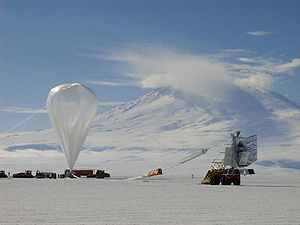
\includegraphics[width=0.30\textwidth]{satellite}
  \end{center}
  \vspace{-20pt}
\end{wrapfigure}
La sonda ha effettuato tre misurazioni nel 1997, 1998 e nel 2003.

\section*{Osservazioni}
\label{osservazioni}

I dati dell'esperimento BOOMERanG del 1997 e 1998, combinati con altri dati riguardanti la costante di Hubble, hanno dato come risultato finale che la geometria dell'universo è piatta. Questo risultato supporta la prova dell'esistenza dell'\emph{energia oscura}. 

I dati del volo del 2003 del BOOMERanG hanno dato come risultato un segnale con un altissimo rapporto segnale-rumore, utili per la mappatura dell'anisotropia della temperatura della radiazione di fondo e per la misura della polarizzazione della radiazione. Inoltre durante il volo antartico del 1998, ripetuto e migliorato nel 2003, le “mongolfiere” di BOOMERanG misurarono per la prima volta le oscillazioni del plasma primordiale, dimostrando l'assenza di curvatura dell'universo e stimando con una accuratezza mai raggiunta prima la densità totale di massa ed energia del cosmo. In questo modo l’esperimento fornì indirettamente la prova che \emph{l’Universo sta accelerando}.

\section*{Curiosità}
\label{curiosit}

L'esperimento BOOMERanG (Balloon Observations Of Millimetric Extragalactic Radiation and Geophysics) è un esperimento che ha misurato la \emph{radiazione cosmica di fondo} di una porzione dello spazio, tramite tre voli sub-orbitali di un pallone di alta quota. Il pallone è stato fatto girare attorno al polo sud sfruttando il vortice polare ritornando così al punto di partenza dopo due settimane, da qui il nome di boomerang.
È stato il primo esperimento in grado di fornire un'immagine ad alta definizione delle anisotropie della temperatura della radiazione cosmica di fondo. L'esperimento ha utilizzato dei \emph{bolometri} per il rilevamento della radiazione di fondo; questi strumenti sono stati mantenuti ad una temperatura di 0,27 K (−272,88 °C). Secondo la legge di Debye i materiali, a tale temperatura, presentano una capacità termica molto bassa; le microonde provenienti dalla radiazione di fondo causano un forte aumento di temperatura, proporzionale all'intensità dell'onda. Queste variazioni di temperatura vengono quindi rilevate da termometri ad alta risoluzione.


\end{document}